% \chapter{Theoretical Backgound}
\chapter{Fundamente teoretice}
\label{cap:fund-teoretice}


In acest capitol sunt evidentiate si explicate pe scurt aspectele teoretice pe care se bazeaza proiectul.

%
%Aici se descriu pe scurt aspecte teoretice pe care se bazează lucrarea. Conținutul acestui capitol trebuie gândit pentru un citor care nu e specializat pe domeniul temei și nu cunoaște chestiunile de bază despre subiect. Pentru un cititor specializat, capitolul poate să stabilească un limbaj comun, relativ la termenii care pot fi interpretați diferit. 
%
%Acest capitol nu trebuie gândit și scris nici ca un copy-paste din alte surse, nici ca zona de reglaj a numărului de pagini ale lucrării. Deși va conține chestiuni pe care le-ați studiat și voi și pe care v-ați bazat, el trebuie să fie o compilare a surselor folosite, care să aibă sens și relevanță pentru lucrarea voastră. Trebuie să fie o descriere coerentă și logică a unor aspecte care ușurează sau fac posibilă înțelegerea părților următoare ale lucrării. Nu trebuie intrat insă prea mult în detalii, ci spuse doar chestiunile esențiale. 
%
%Dacă preluați text, figuri, tabela etc. din sursele de documentare, acestea din urmă trebuie indicate explicit. 
%
%Reprezintă cca. 10--15\% din lucrare.
\section{Reverse proxy}

Un reverse proxy este un server intermediar care trimite mai departe request-urile pentru continut, de la mai multi clienti nedefiniti, catre unul sau mai multe servere. Un reverse proxy este un tip de proxy care in mod normal este situat in spatele unui firewall intr-o retea interna si redirectioneaza traficul clientilor catre serverele asociate. Acesta introduce un nivel in plus de abstractizare si control, asigurand controlul fluxului de trafic \cite{rev_proxy_server}.

\begin{figure}[h]
	\centering
	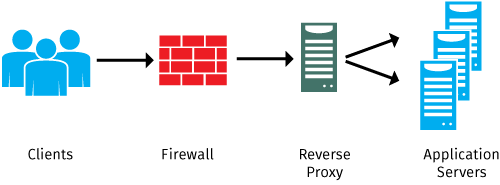
\includegraphics[width=0.6\textwidth]{rev-proxy.png}
	\caption{Folosirea unui reverse proxy in arhitectura unei aplicatii.}
	\label{fig:rev-proxy}
\end{figure}

Figura ~\ref{fig:rev-proxy} prezinta modalitatea de integrare a unui reverse proxy in implementarea arhitecturii de back end a unei aplicatii. \\

Cele mai obisnuite caracteristici ce pot fi oferite de utilizarea unui reverse proxy sunt:
\begin{itemize}
	\item Load balancing - un reverse proxy poate sa distribuie request-urile primite de la clienti, astfel incat nici un server sa nu fie coplesit ce reqesturi. In cazul in care un server este supraincarcat cu reqest-uri sau este cazut, acesta poate sa redirectioneze traficul carea alte servere functionale.
	\item Web acceleration - un reverse proxy poate sa realizeze compresia datelor sau sa memoreze in memoria cache continut ce este frecvent accesat sau poate sa realizeze operatiile de criptare SSL executate in mod normal de server, imbunatatind astfel in mod considerabil viteza de comunicare dintra client si serverul destinatie.
	\item Securitate si anonimitate - prin interceptarea request-urilor primite de catre server, acesta asigura anonimitatea serverului actionand ca un nivel extra de securitate. De asemenea se asigura ca mai multe servere pot fi accesate prin intermediul unui punct comun, indiferent de structura retelei interne.
\end{itemize}



\section{Support vector machine}

Algoritmul de machine learning, support vector machine reprezinta un model obtinut prin folosirea de diversi algoritmi pentru antrenarea acestuia, folosit pentru a clasifica date. Acest model intra in categoria de invatare supravegheata('supervised learning'), intrucat pentru obtinerea lui se foloseste un set de date ca si exemplu, date pe care modelul le va folosi ca referinta pentru clasificarea noilor evenimente.

Realizarea unui astfel de model se obtine in urma executarii unui proces elaborat ce implica mai multi pasi:
\begin{itemize}
	\item  Primul pas reprezinta indentificarea datelor relevante in cea ce priveste problema tratata(setul de antrenare). In conformitate cu scopul clasificarii unor evenimente/ date, in doua(sau mai multe) categorii, initial trebuie indentificate o serie de astfel de evenimente si categorizate de catre utilizator in evenimente ce sigur apartin fiecarei dintre categoriile tinta.
	\item Dupa  obtinerea datelor de antrenare, trebuie indentificate toate trasaturile relevante din aceste date, trasaturi care sa fie cat se poate de specifice fiecarei categorii in parte. Fiind recomandata evitarea trasaturilor ce sunt prezente in mare parte din date sub aceasi forma (ex:caracterul '=' sau'?' intr-un URI folosit pentru clasificarea atacurilor SQL injection), indiferent de categoria din care acestea fac parte.
	\item Dupa obtinerea trasaturilor specifice datelor de antrenare, se realizeaza antrenarea modelului folosind un algoritm specific. In cazul proiectului propus s-a folsoit algoritmul gata implementat, furnizat de biblioteca open source LIBSVM \cite{libsvm}. Pentru obtinerea modelului, datele de antrenare au fost procesate folosind un kernel gausian. Un kernel gausian reprezinta modul in care modelul proceseaza datele de antrenare astfel incat clasificarea noilor date sa fie realizata prin calcularea similaritatilor dintre acestea si cele de antrenare. In calcularea similaritatii dintre aceste doua tipuri de date, un parametru foare important este sigma. Acest parametru este ales pentru intrg setul de date, iar valoarea lui este diret proportionala cu gradul de similaritate pe care algoritmul il va asocia la doua evenimente/date diferite.
\end{itemize}



\begin{figure}[h]
	\centering
	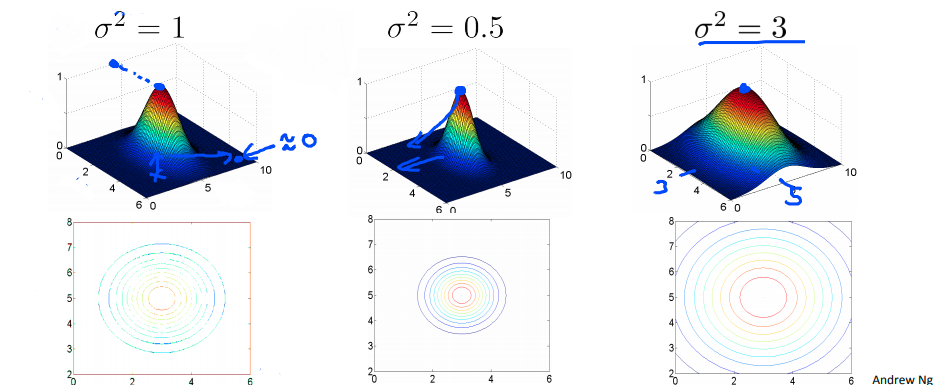
\includegraphics[width=0.8\textwidth]{svm-andrew.png}
	\caption{Influentele aduse algoritmului de modifiacrea parametrului sigma in algoritmul de antrenare.}
	\label{fig:rev-proxy}
\end{figure}


Figura ~\ref{fig:rev-proxy} prezinta cum inflenteaza clasificarea unui nou eveniment valoarea parametrului sigma din formula algoritmului de support vector machine. Figura ~\ref{fig:rev-proxy} a fost preluata din slide-urile cursului de machine leraning sustinut de Andrew Ng \cite{andrew_ng} \\


\section{SQL injection}

Atacurile de tipul SQL injection sunt realizate prin injectarea de cod executabil intr-o baza de date.

Procesul de interactionare cu o baza de date presupene realizarea de interogari asupra acesteia. In formularea acestor interogari, utilizatorul trebuie sa prezinte interpretorului, sub forma de siruri de caractere, numele tabelelor interogate sau valorile unor capuri specifice din acestea. Aceste siruri de caractere sunt delimitate folosind caracterul " sau '. Atacurile de tipul SQL injection expluateaza folosirea acestor delimitatori de siruri de caratere, trimitand siruri de caractere eronate intentionat catre baza de date. Un utilizator rau intentionat poate sa furnizeze astfel de siruri de caractere catre o baze de date prin intermediul oricarui procesator de continut disponibil unui client al unei aplicatii ce comunica cu o baza de date. Aceste siruri de caractere delimiteaza prematur valoarea care este folosita in interogare, introducand dupa aceasta o serie de caractere pe care interpretorul le va trata ca si cod executabil, oferindui astfel utilizatorului sa execute operatiuni asupra bazei de date la care nu ar avea accesul in mod normal. Aceste operatiuni pot sa reprezinte alterarea bazei de date sau obtinerea de date confidentiale. \\



\begin{figure}[h]
	\centering
	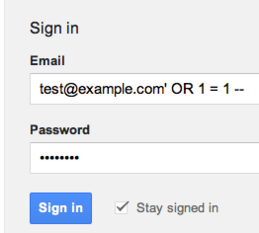
\includegraphics[width=0.4\textwidth]{259px-Sql_Injection_Login.png}
	\caption{Exemplu de atac realizat prin SQL injection.}
	\label{fig:sqli-example}
\end{figure}

Figura ~\ref{fig:sqli-example} prezinta o tenatativa de atac prin SQL injection in care in campul de validare a email-ului se incearca injectarea de cod ce va fi executat in interogarea de validare a credentialelor. Prin prezenta caracterului ' se escapeaza tot textul urmat dupa acesta ca fiind cod si nu un string ce face parte din campul de email. Operatia logica "OR 1=1" va determina interpretorul sa returneze adevarat(valid) pentru orice adresa de email introdusa introdusa inaintea caractrului '. \\


\section{Adresele IP ale retelei Tor}
Reteaua Tor reprezinta un softrware gratis de anonimizare a traficului pe internet. Numele este de fapt un actonim pentru "The Onion Router"(router-ul ceapa) care sugereaza modul de functionarea al acestuia, ficare nod din retea adugand un strat extra de securitate celor precedente. Modul de functionare al retelei se bazeaza pe rutarea traficului prin cat mai multe noduri pentru a anonimiza si a face cat mai greu de urmarit traficul unei anumite persoane. Aceste noduri prin care traficul este directionat sunt sustinute gratis de catre voluntari/utilizatori de Tor din intreaga lume.

Pentru criptarea traficului reteaua Tor foloseste criptarea la nivelul aplicatiei in cea ce priveste sructura retelelor de calculatoare(modelul OSI sau TCP/IP). Datele trasmise sunt criptate, incluzand destinatia, cu exceptia nodului urmator, astfel creandu-se structura de "ceapa" asupra unui pachet. Selectia nodurilor prin care se face rutarea pachetelor este aleasa random. Fiecare pachet decripteaza un "strat", afand nodul urmator pentru pachetul respectiv, nodul final decriptand datele initiale si realizand trasmisia catre destinatie, fara sa ii comunice sursa pachetului. Intrucat in comunicarea pachetelor, pe parcursul rutelor parcurse, se cunoaste in permanenta doar nodul urmator, acest lucru impiedica monitorizarea traficului intre sursa si destinatie.


Cu toate ca reteua tor ofera anonimitate de partea clientului, acest lucru nu se realizeaza si fata de ea. Reteaua nu se ascunde fata de serviciile acesate prin intermediul ei. Astfel un site anume poate sa detecteze daca un anumit client il acceseaza folosind reteaua Tor sau nu.

Intrucat reteaua Tor nu isi ascunde adresele IP folosite de catre aceasta, indentificarea lor si procurarea de date despe acestea este destul de usoara. In proiectul propus s-a folosit un serviciu care furnizeaza gratui astfel de date \cite{tot_status}(adresa IP, uptime etc.) si s-au folosit algoritmi propri pentru procesarea acestor date, eliminand astfel necorectitudinea dintre utilizatorii retelei.

\begin{figure}[h]
	\centering
	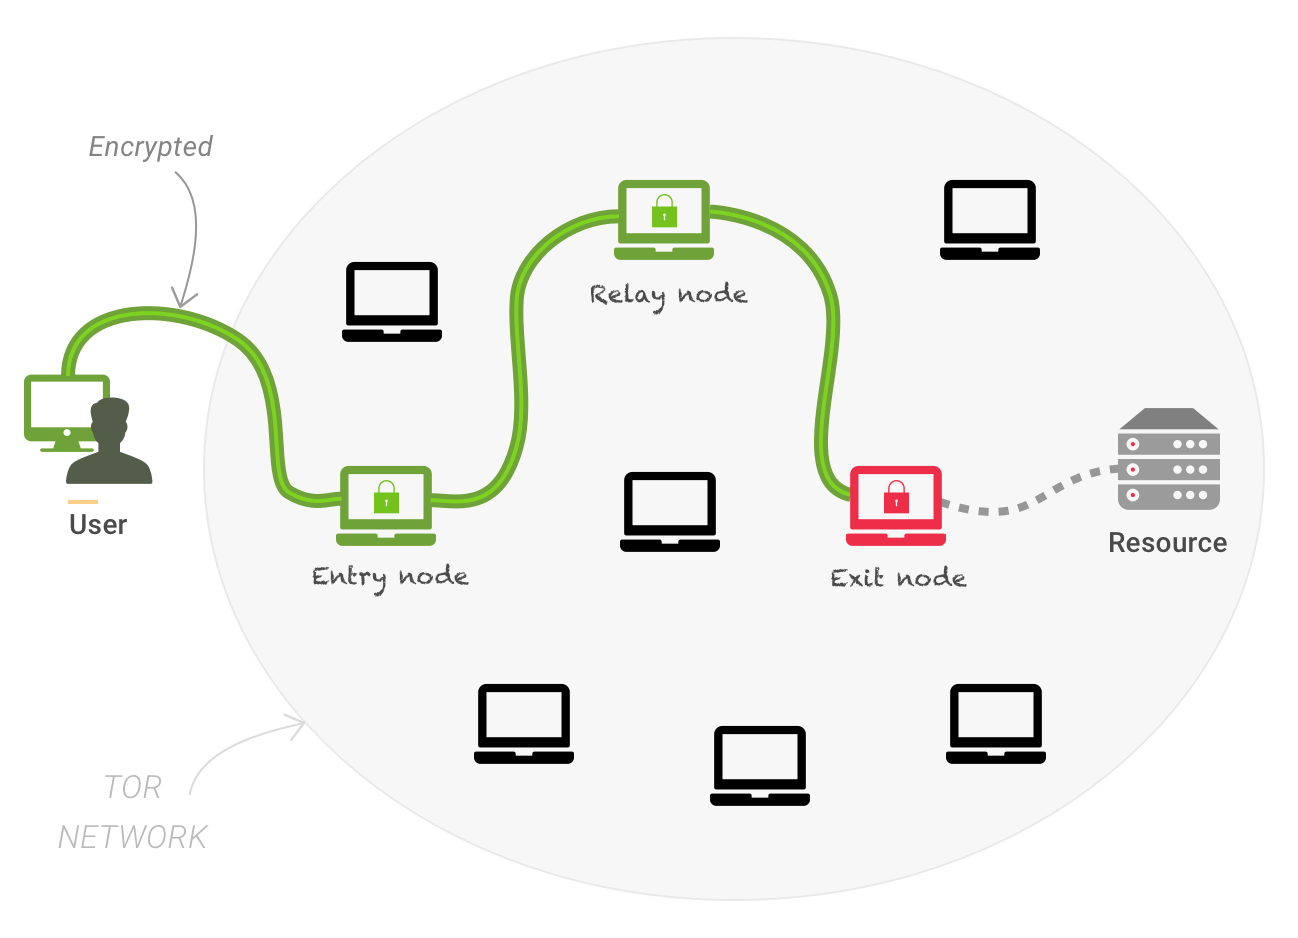
\includegraphics[width=0.6\textwidth]{can-you-hide-on-Tor-Network.png}
	\caption{Exemplu de trafic realizat prin reteaua Tor.}
	\label{fig:tor-example}
\end{figure}

Figura ~\ref{fig:tor-example} prezinta principalele elemente folosite la rutarea treficului de la client la destinatie prin intermediul retelei Tor. \\


\section{Sistem de prevenire a intruziunilor}
Conform scurtei descrieri prezentate in capitolul anterior, un sistem de prevenire a intruziunilor are rolul de a filtra traficul dintre clientii unui server si serverul propiu zis. 

Acest sistem functioneaza liniar, adica este plasat direct intre server si clienti acestuia. In cazul proiectului propus, componenta de baza pentru interceptarea traficului este realizata prin implementarea unui reverse proxy, oferind astfel caracteristica de interceptare si decriptare a traficului, ce permite analiza acestuia, dar si avantajele specifice utilizarii unui reverse proxy.

Pentru filtrarea traficului, un sistem de prevenire a intruziunilor implementeaza anumiti senzori care au rolul sa inspecteze tot traficul ce trece prin sistem, realizand aceasta inspectie in timp real. Datorita acestei verificari, orice pachet considerat malitios este oprit din a ajunge la serverul destinatie. In proiectul propus, implementarea acestor senzori este realizata in doua moduri. In cazul validarii adreselor IP impotriva utilizatorilor de Tor se folosete o lista de IP-uri ce contine adrese frecvent utilizate de reteaua Tor. In interiorul reverse proxy-ului, in momentul crearii unei noi conexiuni, acesta verfica ca adresa IP ce solicita conectarea la server sa nu fie continuta de lista mentionata. In cazul detectiei impotriva atacurilor de SQL injection, senzorul este implementat utilizand un model de support vector machine. In interiorul reverse proxy-ului in momentul interceptarii unui request venit din exterior catre reteaua interna, acesta verifica daca reqestul poate fi clasificat ca si tentativa de atac. In caz afirmativ blocand trecerea acestuia mai departe catre server.
\begin{figure}[h]
	\centering
	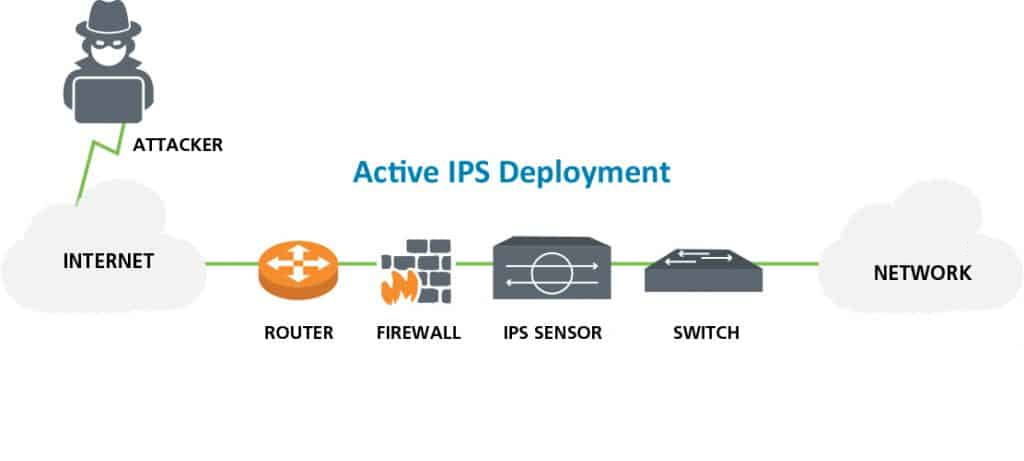
\includegraphics[width=0.6\textwidth]{IPS.png}
	\caption{Integrarea unui sistem de prevenire a intruziunilor intr-o retea.}
	\label{fig:ips-2nd-example}
\end{figure}

Figura ~\ref{fig:ips-2nd-example} prezinta arhitectura unei retele interne ce integreaza un sistem de prevenire a intruziunilor pentru protejarea acesteia. \\

Un sistem de prevenire a intruziunilor poate sa efectueze oricare din urmatoarele actiuni in momentul detectarii unui eveniment malitios \cite{ips_fire}:
\begin{itemize}
%	Terminates the TCP session that is being exploited by an outsider for the attack. It blocks the offending user account or source IP address that attempts to access the target host, application, or other resources unethically.
	\item Sa intrerupa sesiunea dintre client si server, in cazul in care clientul desfasoara sau incearca sa desfasoare activitati malitioase in reteaua protejata de sistem. Acest lucru se poate realiza prin blocarea anumitor credentiale asociate cu utilizatorul respectiv sau prin blocarea adresei IP a acestuia.
	\item In conditiile in care un sistem de prevenire a intruziunilor detecteaza/clasifica o activitate ca fiind malitioasa, acesta poate sa ia masuri automat pentru a preveni un astfel de atac pe viitor(ex: in momentul detectarii unei tentative de atac prin SQL injection, sistemul de prevenire a intruziunilor poate sa blocheze in mod automat adresa IP a utilizatorului ce inceraca sa faca atacul, nepermitandu-i acestuia sa se mai conecteze la serverul destinatie pentru un anumit interval de timp sau pana la interventia unui administrator).
	\item O alata abordare posibila in momentul declansarii unui eveniment malitios este alterarea traficului astfel incat sa elimine continutul malitios din acesta. Pentru realizarea acestui lucru, un sistem de prevenire a intruziunilor poate sa stearga atasamente infectate din interiorul unui mail, sa altereze continutul unui pachet sau sa omita trasmiterea mai departe a unor pachete.
	
\end{itemize}

